\subsection{System Overview}

\begin{figure}
  \centering
  % Requires \usepackage{graphicx}
  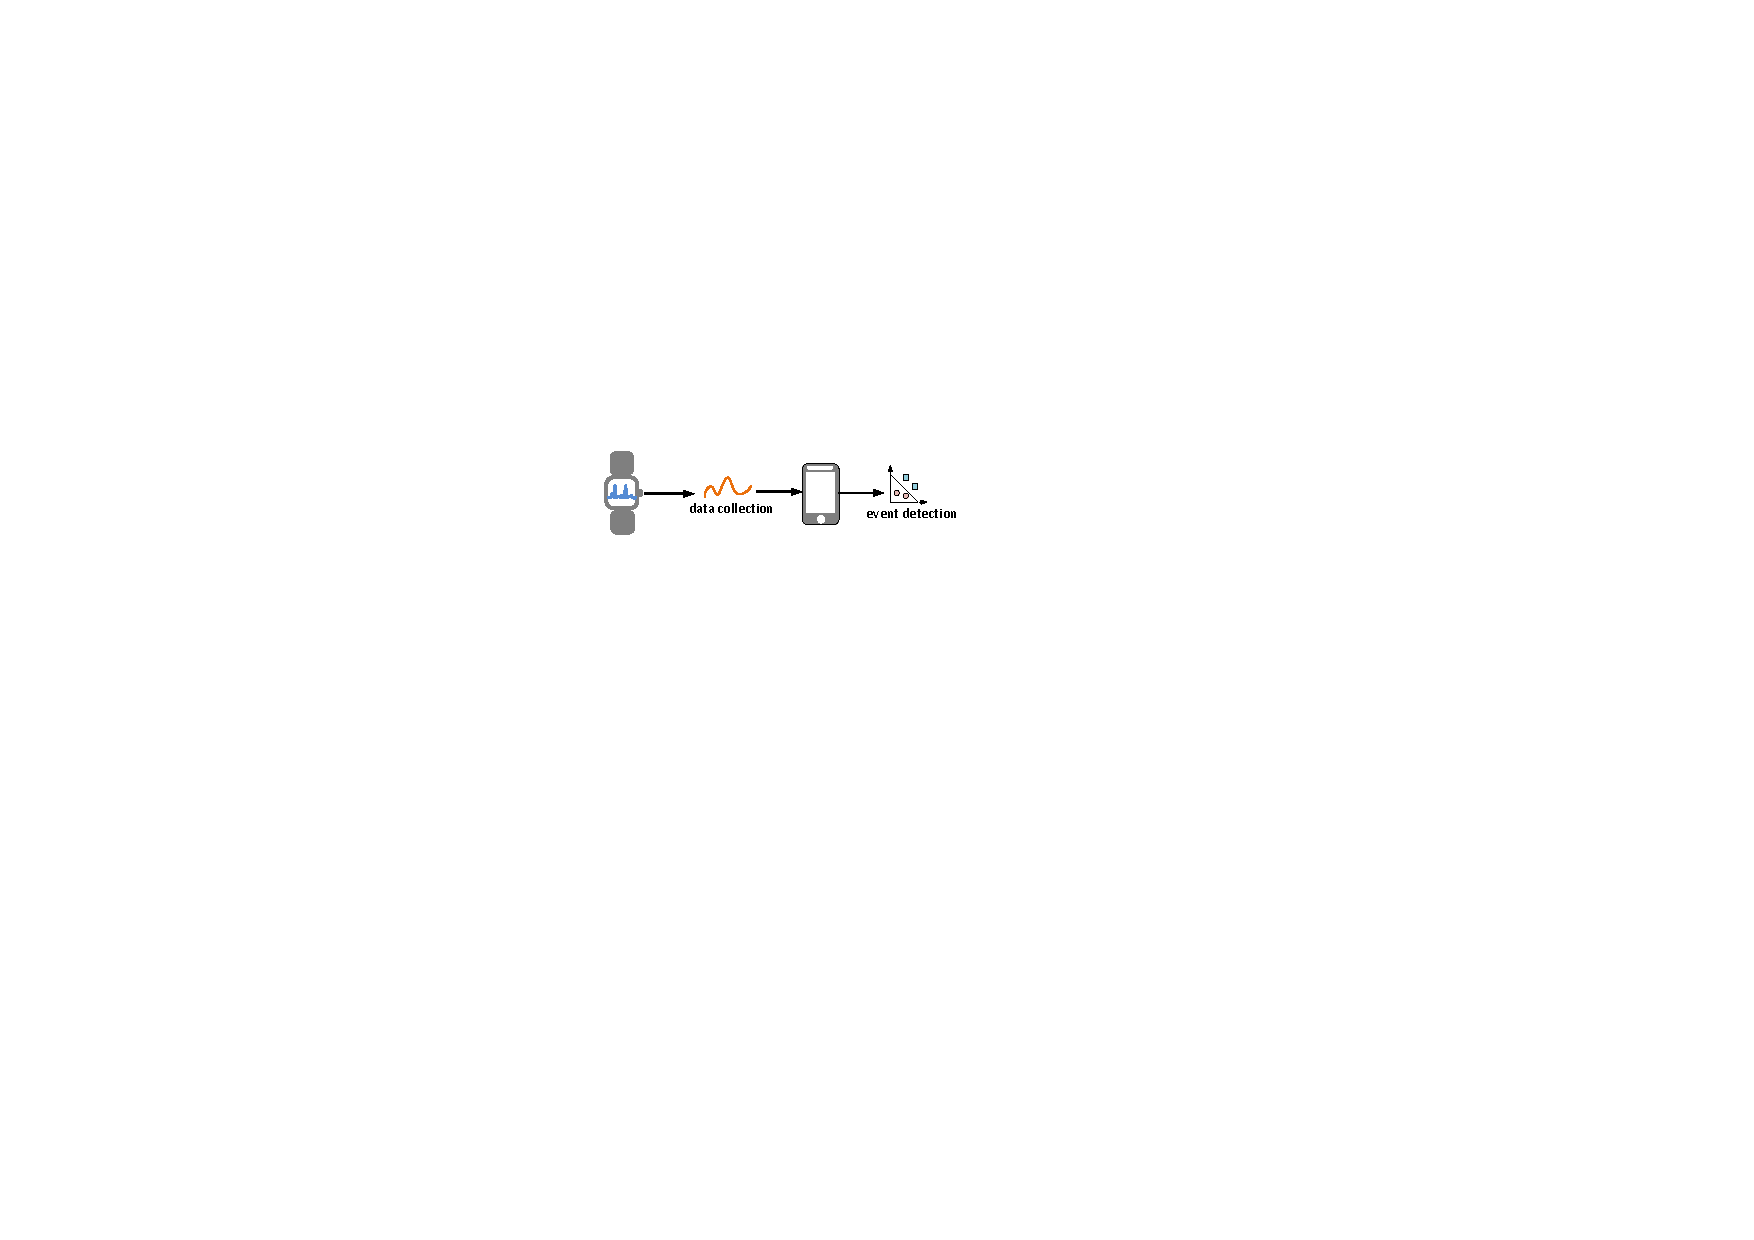
\includegraphics[width=0.7\textwidth]{figures/overviewd.pdf}\\
  \caption{Overview of our 2-stage approach. Sleep data are collected through smartwatch sensors, which are then passed to be processed by a mobile app
  to detect sleep events.}\label{fig:overview}
\end{figure}

Figure~\ref {fig:overview} depicts our 2-state approach that involves collecting data using a smartwatch and sleep event detection using a
smartphone. Sleep data are collected using smartwatches sensors. Our work exploits a wide range of sensors that are common on commercial
off-the-shelf smarwatches. Specifically, we use the accelerometer and gyroscope to collect body movement data, the microphone to measure
acoustic data, the ambient light sensor for illumination conditions, the orientation sensor for calibration. The collected data are
transmitted to a smartphone via Bluetooth. We propose a set of new analysis and algorithms to effectively detect sleep events from the
collected data. Table~\ref{tab:test} lists the set of sleep events supported by \systemname.

\begin{table}[t!]
 \caption{\label{tab:test}Sleep events targeted in this work}
 \centering
 \begin{tabular}{ll}
  %\toprule
  \toprule
  \textbf{Event}& \textbf{Type} \\
  \midrule
\rowcolor{gray}  Sleep postures & Supine, Left lateral, Left lateral, Prone\\
 Hand positions & Head, Chest, Abdomen\\
\rowcolor{gray} Body rollover & Count\\
 Micro body movements& Hand moving, Arm raising, Body trembling \\
\rowcolor{gray} Acoustic events & Snore, Cough, Somniloquy  \\
 Illumination condition & Strong, Weak  \\
  \bottomrule
 %\hline
 \end{tabular}
\end{table}

%\begin{figure}[!thbp]
%\centering
%%\setlength{\belowcaptionskip}{-9pt}
%      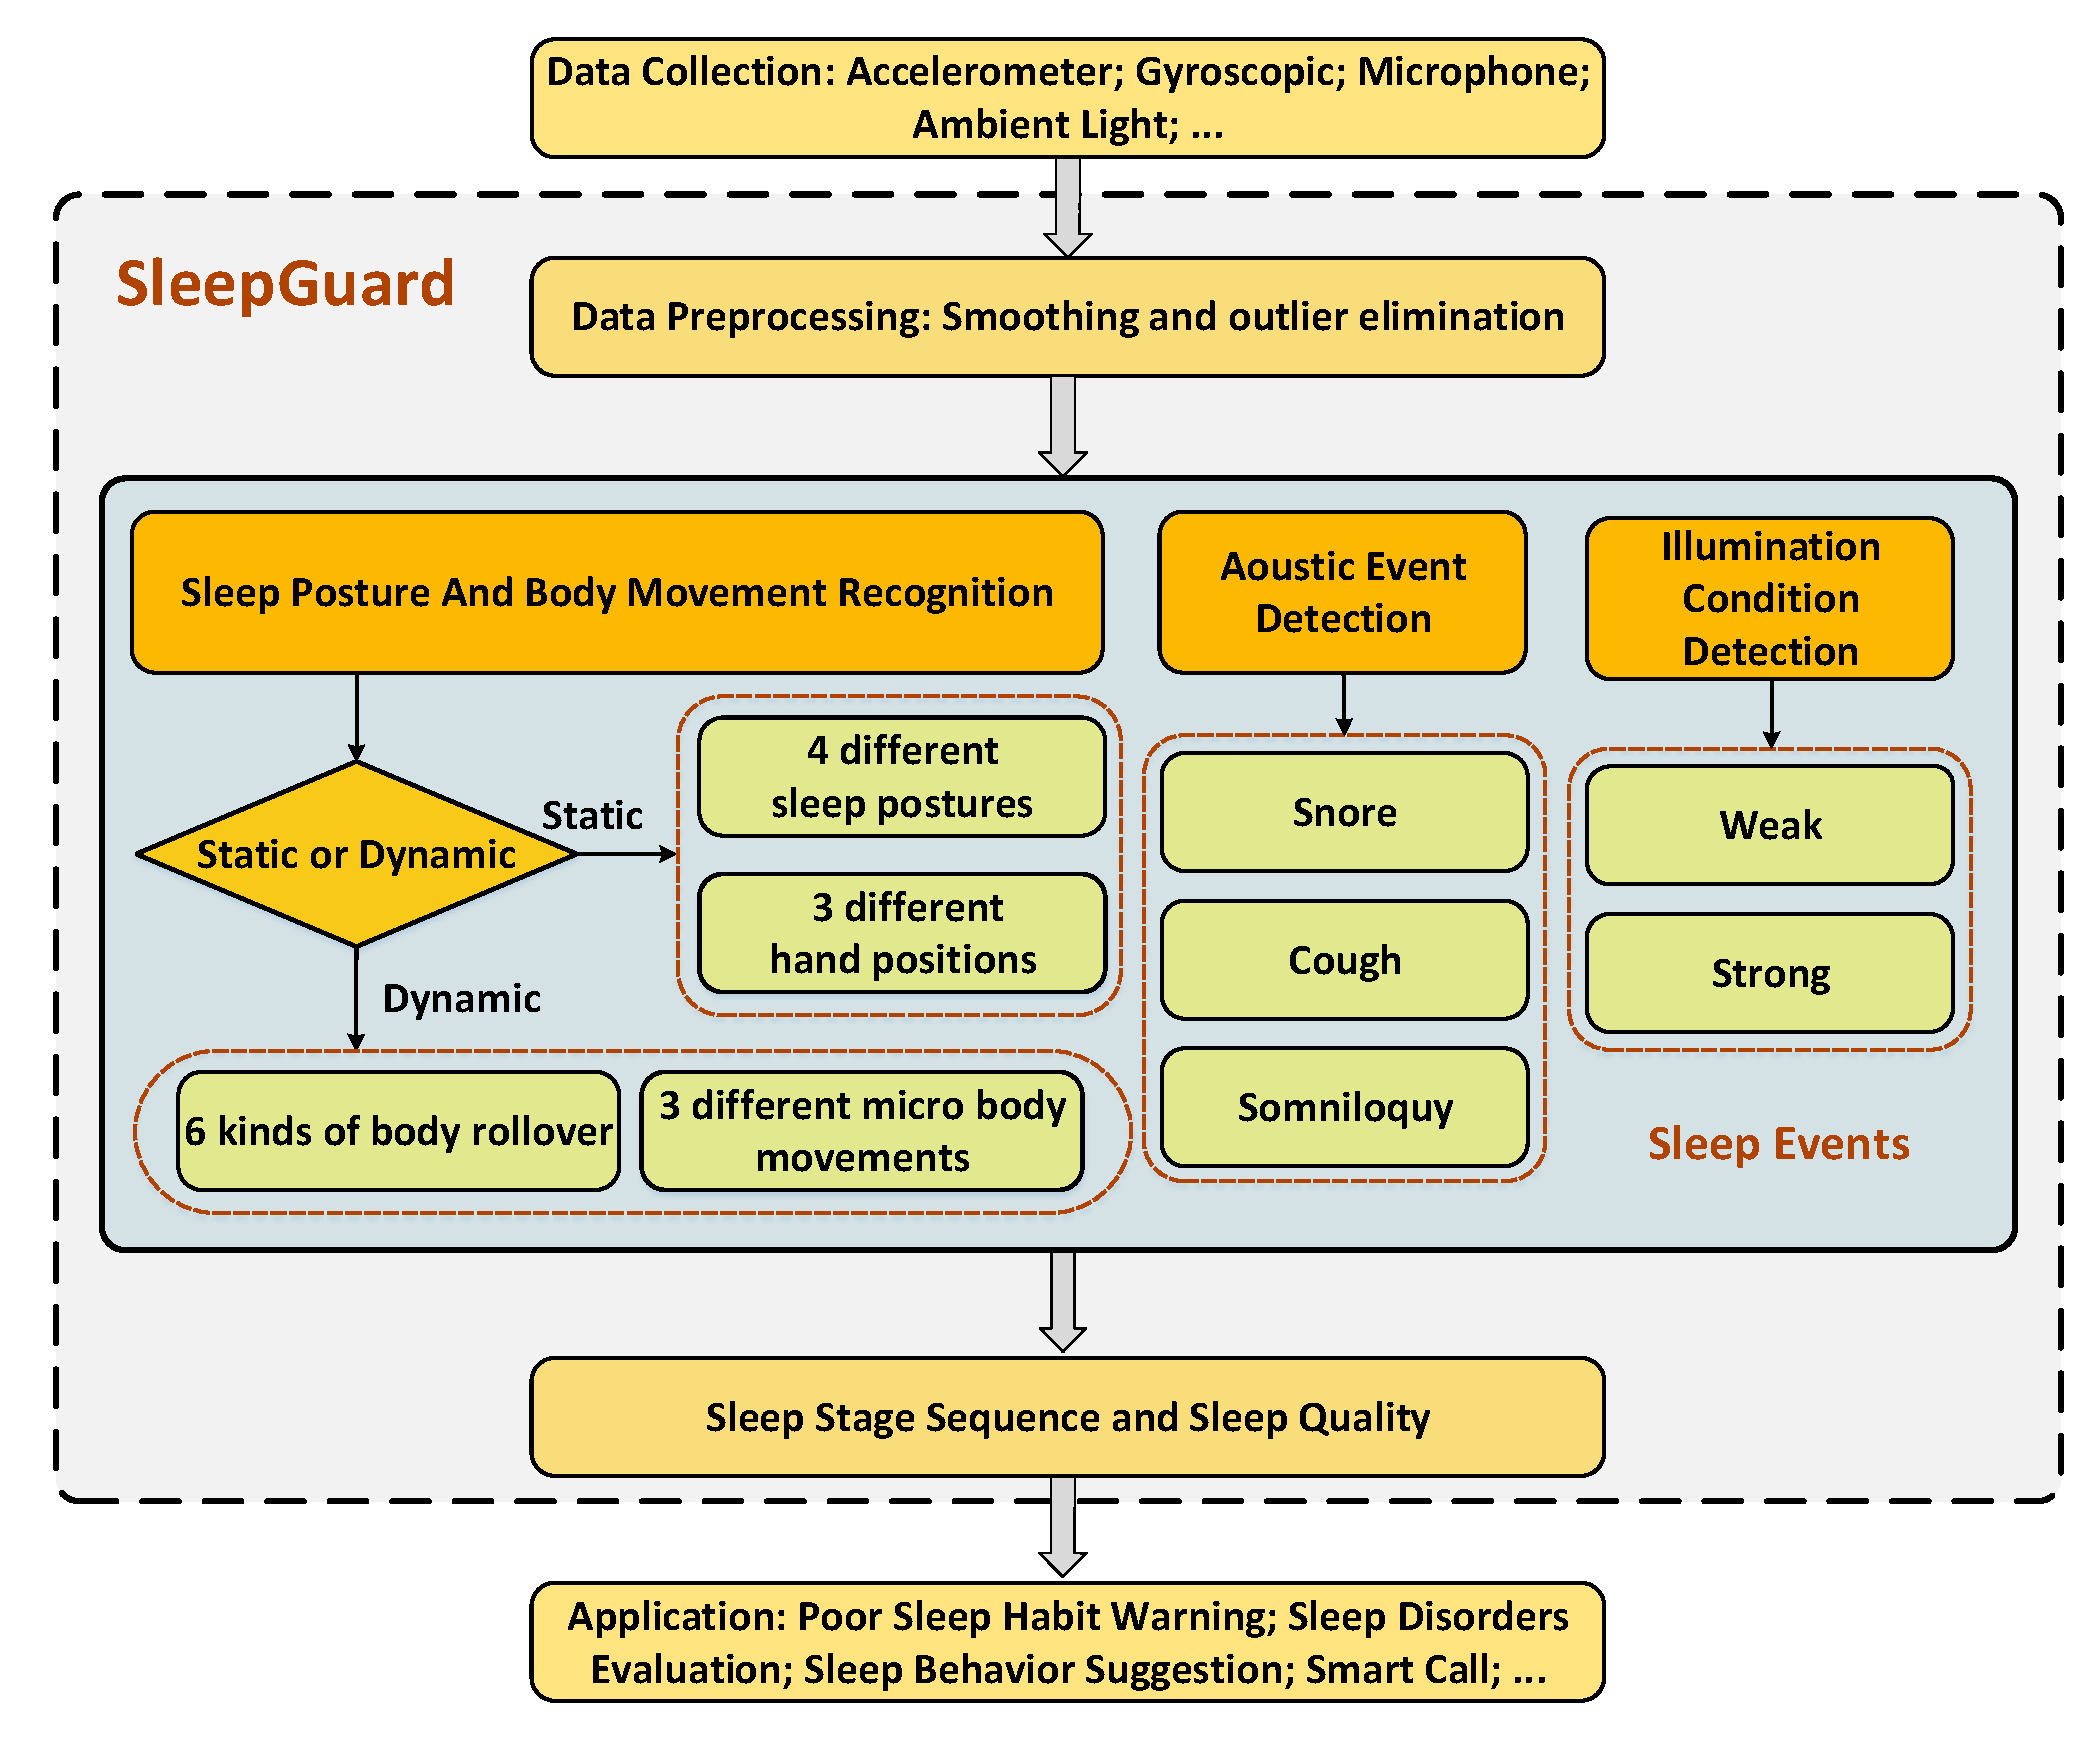
\includegraphics[width=0.97\linewidth]{Figures/SystemFlow.pdf}
%  \caption{System overview of {\systemname}.}\label{fig:overview}
%\end{figure}
%
%
%\begin{itemize}[itemsep=1mm,nolistsep]
%  \item {\textbf{Data Collection and Preprocessing.}} A variety of sensing data are related to sleep events include i) the accelerometer and the gyroscope about the body movement, ii) the microphone measured acoustic sound, iii) the ambient light sensor about the illumination condition, and iv) the orientation sensor with some auxiliary information. The data is collected every 30 ms on the smartwatch and transferred to the server (such as a smartphone) via Bluetooth. We use data smoothing and outlier elimination to reduce noise in the raw sensor readings.
%  \item \textbf{Sleep Event Detection.} A series of novel algorithms are developed to recognize different sleep events. In particular, some key insights are observed about different body postures, body rollovers, hand positions, micro body movements and acoustic events. Note that before identifying those events, {\systemname} first carries out a coarse-grained detection and judges whether the user is lying or not.  After that, we can estimate the user's bedtime. During the user is lying on the bed,  we regard that the user fell asleep if we do not detect a large movement within 20 minutes.
%  \item \textbf{{Sleep Pattern Report.}} Sleep Pattern Report. After we obtain the detected sleep events, we integrate them to the clock information, illumination condition, and then use the Hidden Markov Model to infer the sleep stages and evaluate sleep quality. Different from existing apps on the market, {\systemname} provides detailed procedure about the sleep report. The output of our system, for example, sleep postures and the position of user's hand could be used as input to build a broad range of sleeping quality and  heathy applications, such as poor sleep habit warning, the evaluation of insomnia, nightmare and sleep disorders. With the extensive experiments conducted, we conclude that {\systemname} exhibits a relatively high accuracy comparing to state-of-the-art systems.
%\end{itemize}


%\subsection{Feature Calculation and Selection}
%Appropriate  features  can  reflect  the  potential  information  underlying the  signals. The  features  used  in {\systemname} are shown in  Table \ref{Tab1}. To detect different sleep events, we use two main features. The first one is the movement related features, that are angle of inclination calculated by acceleration data and the angle of rotation calculated by gyroscopic data. Beyond that, to detect different sound events during sleep, we calculate the energy and zero-crossing rate of the sound signal.
%
%\begin{table}[!thbp]
%\centering
% \caption{Calculated Features}\label{Tab1}
%   \renewcommand\arraystretch{1.7}{\multirowsetup}{\centering}
%        \begin{tabular}{c|c|c}
%        \hline
%        {\bf{Data}}  &   {\bf{Feature}} &   {\bf{Formula}}\\
%         \hline
%        {$acc$} & {Tilt Angle}   & $ A_x =\arccos(\frac {acc_x}{acc}) $ \\
%        \hline
%        {$\omega$} &  {Rotation Angle}  & $ \theta = \int\omega $ \\
%        \hline
%        %\multirow{2} {0.1cm}
%        {Sound}  & Energy   &$ E=\sum\nolimits_{n=-\infty}^{\infty}|x^2(n)|$ \\
%         {$x(n)$}  & Zero-crossing  & $Z$ \\
%          \hline
%\end{tabular}
%\end{table}
